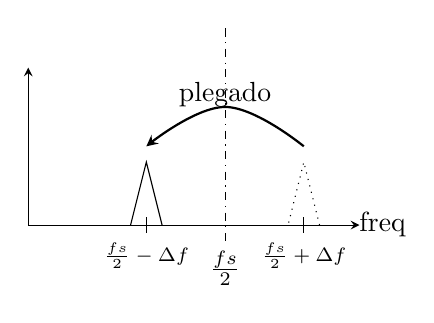
\begin{tikzpicture}
\tikzstyle{invisible} = [outer sep=0,inner sep=0,minimum size=0]
\tikzstyle{stealth} = [-stealth]
\node [invisible] (v1) at (0,0) {};
\node [invisible] (v2) at (0,2) {};
\node [invisible] (v3) at (4.5,0) {freq};
\draw [stealth] (v1) edge (v2);
\draw [stealth] (v1) edge (v3);
\draw [dashdotted](2.5,2.5) -- (2.5,-0.2) node[anchor=north]{$\frac{fs}{2}$};

\draw [invisible, dotted](3.7,0) node [circle] {} -- 
				 (3.5,0.8) node [circle] {} -- 
				 (3.3,0) node [circle] {};
\draw [draw](3.5,0.1) -- (3.5,-0.1) node[anchor=north]{\scriptsize$\frac{fs}{2} + \Delta f$};
\draw [invisible](1.7,0) node [circle] {} -- 
			     (1.5,0.8) node [circle] {} -- 
			     (1.3,0) node [circle] {};
\draw [draw](1.5,0.1) -- (1.5,-0.1) node[anchor=north]{\scriptsize$\frac{fs}{2} - \Delta f$};
\draw [invisible, thick, stealth] plot[smooth, tension=.7] coordinates {(3.5,1) (2.5,1.5) (1.5,1)};
\node [invisible, anchor=south] at (2.5,1.5) {plegado};
\end{tikzpicture}